% !TEX root = ../thesis.tex
\section{Analýza dat a první modely}
\label{chap:experiments:analysis}

Rozpoznávání řeči se věnuje nemalé usílí již od 50. let 2O. století a v současné době nikoho nepřekvapí téměř bezchybně fungující obecný rozpoznávač v mobilních zařízeních. Pro obecné systémy dokonce existují korpusy s desítkami ne-li stovkami a více hodin promluv, které je možné využít při vytváření těchto systémů.

Tyto korpusy však obsahují vě většině případů pouze \uv{standardní}\footnote{Slovením spojením \uv{standardní řeč} je myšlena řeč neobsahující vyrazné řečové vady, případně jiné formy produkce a často v nepřílíš akusticky náročném prostředí.} řeč. Pokud je snaha vytvořit nebo ověřit funkčnost systému za specifických podmínek (ať už se jedná o rušné prostředí či speciální typy promluv), tak je nezbytné získat potřebná data.

\subsection{Vytvoření korpusu EL promluv}

Na začátku všeho je idea, v tomto případě o pomoci skupině lidí mající problémy s přirozenou řečí. Vůbec prvním předpokladem, na cestě k úspěšnému dosažení vůbec nějakého cíle, jsou data. Jelikož se jedná o velmi spefická data, tak je potřeba zajistit co možná největší množství kvalitních\footnote{Kvalitou je myšlena věrnost dat dané doméně dále se mluví o přesnosti ve smyslu bezchybnosti přepisů.} a přesných dat.

V části \ref{sec:cause:desease} bylo zmíněno, že ročně se objevý více než 100 nových případů trvalé ztrázy hlasu ročně. Zaroveň bylo řečeno \cite{Skvrnakova2010}, že více rizikovými osobami jsou starší lidé, kteří intenzivně kouří a konzumují alkohol. Přesto je velmi patrný trend nárůstu mladších pacientů a tím i případnému nárůstu případů ztráty hlasu. Přičteme-li již zmíněný psychologický aspekt jeho ztráty, tak je zřejmé, jak komplikované je získat ke spolupráci i jen jednoho řečníka ochotného podstoupit naročné\footnote{I pro zdravého člověka je někdy někalikahodinové nahrávání vysilující. Pro jedince po TL to je z mnoha důvodů ještě řádově náročnější.} nahrávání.

Při libovolné práci s pacienty po TL, dřív nebo později dojde k určité formě spolupráce s oddělením ORL, které má nastarosti péči o tyto pacienty. V našem připadě nejprve s ORL klinikou při Fakultní nemocnici v Plzni a poté i s ORL klinikou Fakultní nemocnice v Motole. S jejich pomocí jsme získali ke spolupráci jednoho řečníka. Konkrétně se jedná o dámu v duchodovém věku, která podstoupila TL před více než 15 lety. Po překonání ostychu\footnote{Podle jejích vlastních slov nebyla schopna několik let po operaci ani zvednout nečekaný telefonní hovor natož mluvit na veřejnosti.} se byla schopna naplno vrátit do běžného života a dokonce v určité formě opět přednášet o stomatologii na Lekařské fakultě v Plzni Univerzity Karlovy.

S její pomocí jsem, v 1. etapě nahrávání, byli schopni pořídit přes 10 hodin promluv, viz tabulka \ref{tab:experiments:analysis:recording}. Nahrávání probíhala v relativně spartánských podmínkách v běžných prostorách katedry za plného provozu. K nahravání byl použit profesionální mikrofon (\todo{typ mikrofonu}{TBD}), ale mezi ostatními komponentami byla již běžná externí zvuková karta a soukromý notebook. Celé nahrávání bylo rozděleno do 14 samostatných sezení a probíhalo od prosince roku 2010 do května roku 2011. Každé sezení trvalo přibližně dvě hodiny během kterých jsme byli schopni získat necelou hodinu akustických dat. Samotné nahrávání se sestávalo z 10 - 20 minutového úseku pořizování nahrávky a přibližně 10 minut dlouhého odpočinku. Ten byl nezbytný z důvodu únavy řečníka.

Pro potřeby nahrávání byly vytvořeny 2 sady vět:

\begin{enumerate}
  \item sada obsahující všechny fonémy - \textit{40 vět}.
  \item sada obsahující věty s reálnou četností fonémů - \textit{5000 vět}.
\end{enumerate}

\noindent Pořízené nahrávky vždy odpovídají 10 - 20 minutovému úseku nepřerušovaného nahrávání a soubory tak vždy obsahují několik vět, které jsou od sebe odděleny minimálně 5 sekundovým úsekem ticha. Nahrávky dále mouhou obsahovat opakování chybně vyslovené věty, přeřeknutí, kýchnutí a další neřečové události.

Přestože byly nahrávky pořízeny na základě předpřipravených sad vět, bylo nezbytné je anotovat. Ještě před samotným anotováním byly nahrávky, podle úseků s tichem, rozsekány na menší části. Jelikož řečník mohl, např. kvůli potřebě hlubšího nádechu nebo úpravě pozice EL, udělat pauzu i uprostřed věty, je výsledný počet souborů vyšší\footnote{Zvýšení je způsobeno i faktem, že ne všechny věty se podařilo nahrát na první pokud. Celkově se tímto zvýšil počet souborů o $5 - 10 \%$.} než skutečný počet nahraných vět, viz tabulka \ref{tab:experiments:analysis:recording}. K anotaci posloužil interní nástroj určený k tomuto účelu a podíleli se na něm celkem 3 anotátoři z řad studentů, kteří si vzájemně kontrolovali své anotace. Ačkoli bylo potřeba anotovat relativně malé množství dat (cca 10 hodin audio záznamu), tak anotace zabrala přibližně 2 měsice. Hlavním důvodem byla relativně dlouhá doba, po kterou se anotátoři adaptovali na specificka EL řeči. Hlavním problémem bylo to, že nejprve nebyli vůbec schopni poruzumnět obsahu promluvy a tím pádem jej správně přepsat.

Výsledný korpus představuje $5040$ unikátních vět rozdělených do $6385$ souborů (viz tabulka \ref{tab:experiments:analysis:recording}), které v průmeru obsahují $7$ slov o průmerné délce $5$ znaků. Tento korpus poslouží jako základ pro všechny budoucí experimenty.

\begin{table}[htpb]
  \centering
  \def\arraystretch{1.5}
  \pgfplotstabletypeset[
    col sep=comma,
    string type,
    columns/phase/.style={column name=Nahrávání, column type={|l}},
    columns/length/.style={column name=Délka \textit{[HH:MM:SS]}, column type={|r}},
    columns/sentences/.style={column name=Počet vět, column type={|r}},
    columns/files/.style={column name=Počet souborů, column type={|r|}},
    every head row/.style={after row=\hline, before row=\hline},
    every last row/.style={after row=\hline},
  ]{./ch4-experiments/tabs/02-recording1-stats.csv}
  \caption{Infoemace o korpusu nahrávek z 1. etapy nahravání.}
  \label{tab:experiments:analysis:recording}
\end{table}

\subsection{Analýza získaných dat}

\begin{figure}[hbpt]
  \centering
  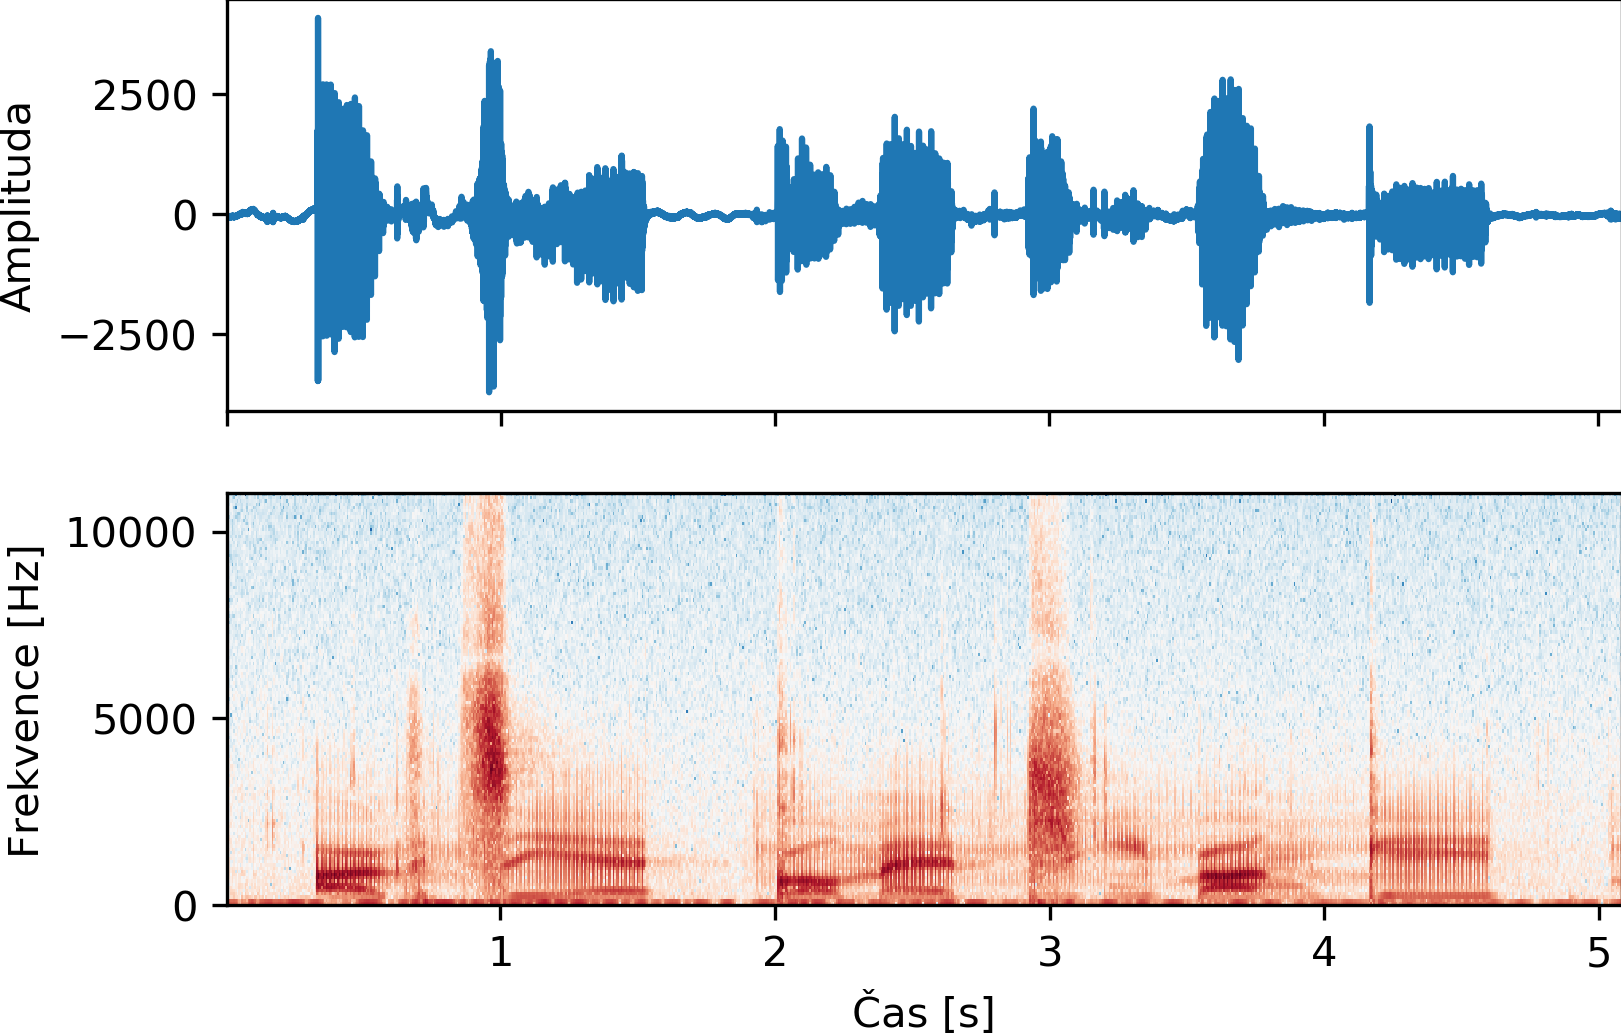
\includegraphics[width=0.8\textwidth]{./ch4-experiments/img/speaker1.png}
  \caption{Průběh a spektrogram promluvy \uv{Akcie komerční banky}.}
  \label{fig:experiments:analysis:speech}
\end{figure}

\begin{figure}[htpb]
  \centering
  \begin{subfigure}[b]{0.4\textwidth}
    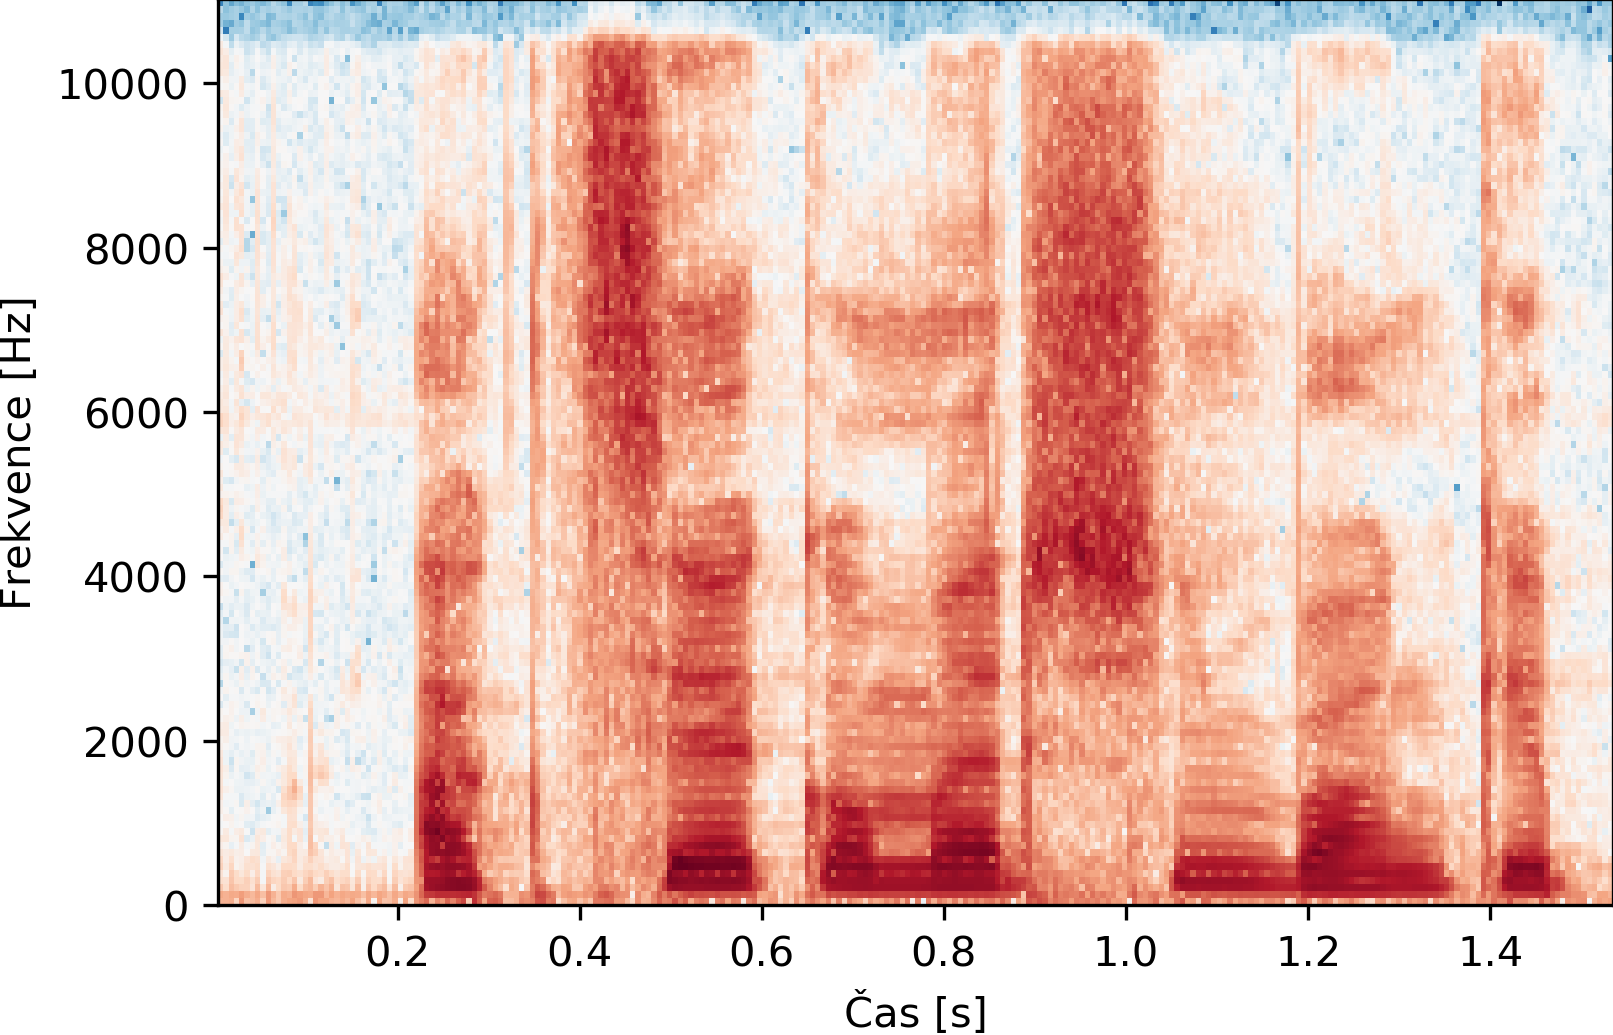
\includegraphics[width=\textwidth]{./ch4-experiments/img/spectrogram0.png}
    \caption{Zdravý řečník}
    \label{fig:experiments:analysis:spectrogram:normal}
  \end{subfigure}
  %
  \begin{subfigure}[b]{0.4\textwidth}
    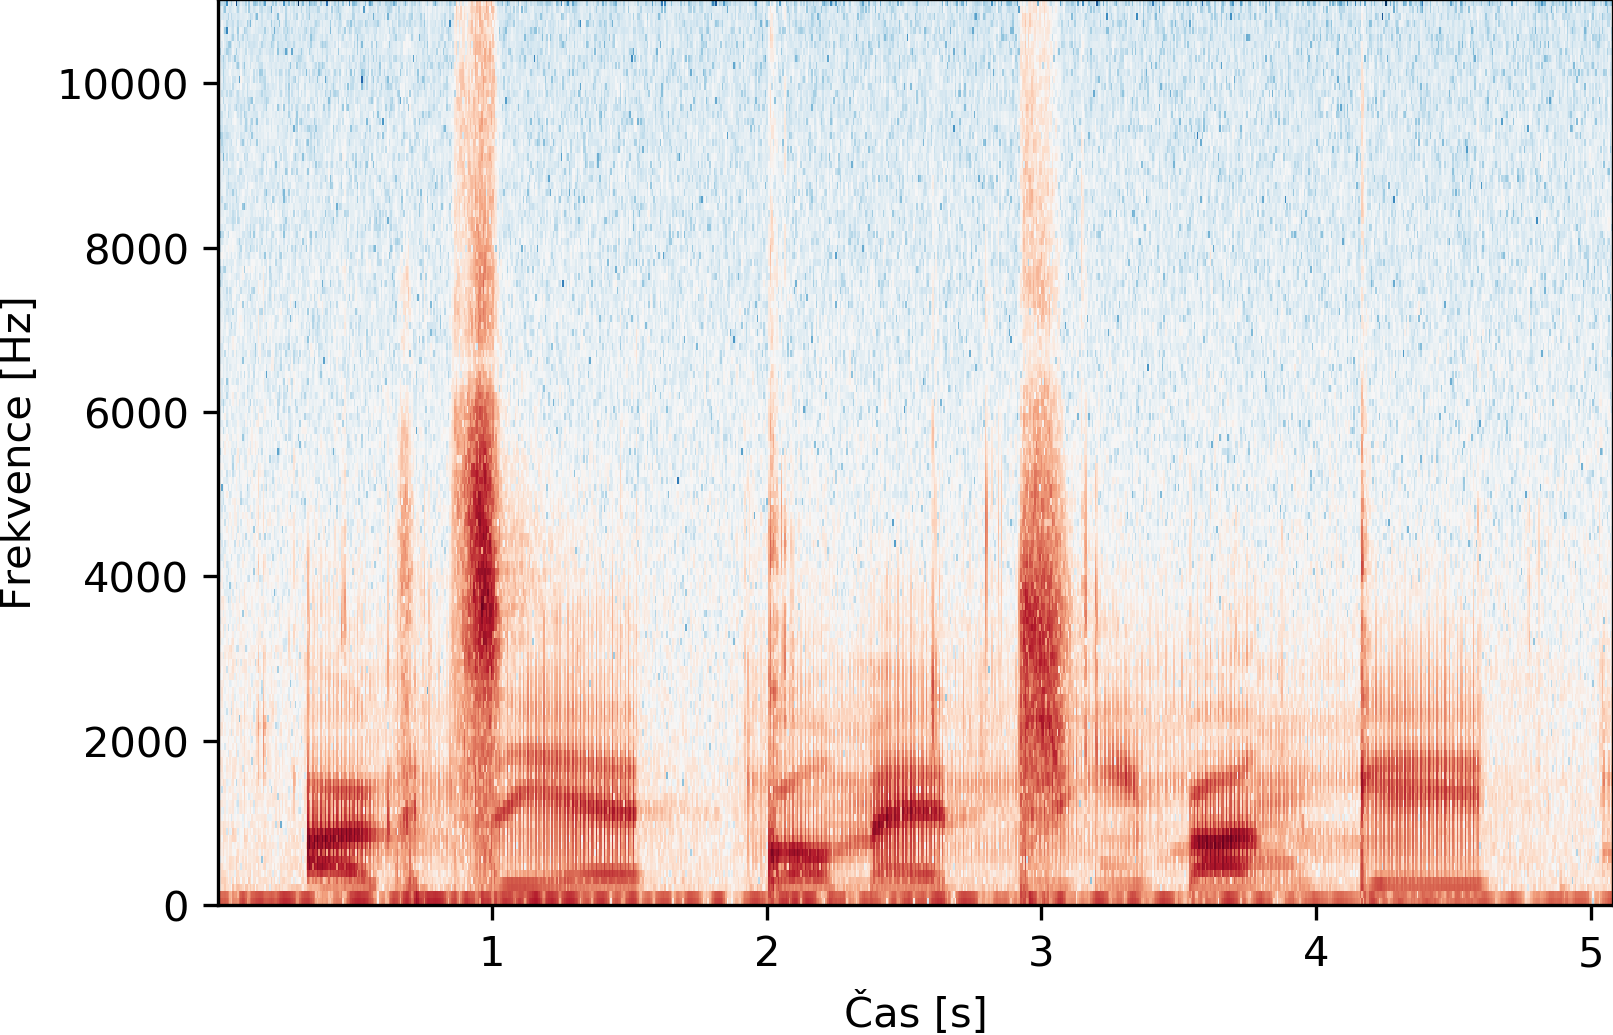
\includegraphics[width=\textwidth]{./ch4-experiments/img/spectrogram1.png}
    \caption{EL řečník}
    \label{fig:experiments:analysis:spectrogram:el}
  \end{subfigure}
  \caption{Spektrogram promluvy \uv{Akcie Komerční banky} dvou řečníků.}
  \label{fig:experiments:analysis:spectrogram}
\end{figure}

test \ref{fig:experiments:analysis:spectrogram} \ref{fig:experiments:analysis:spectrogram:el} \ref{fig:experiments:analysis:spectrogram:normal}

% \begin{figure}[]
%   \centering
%   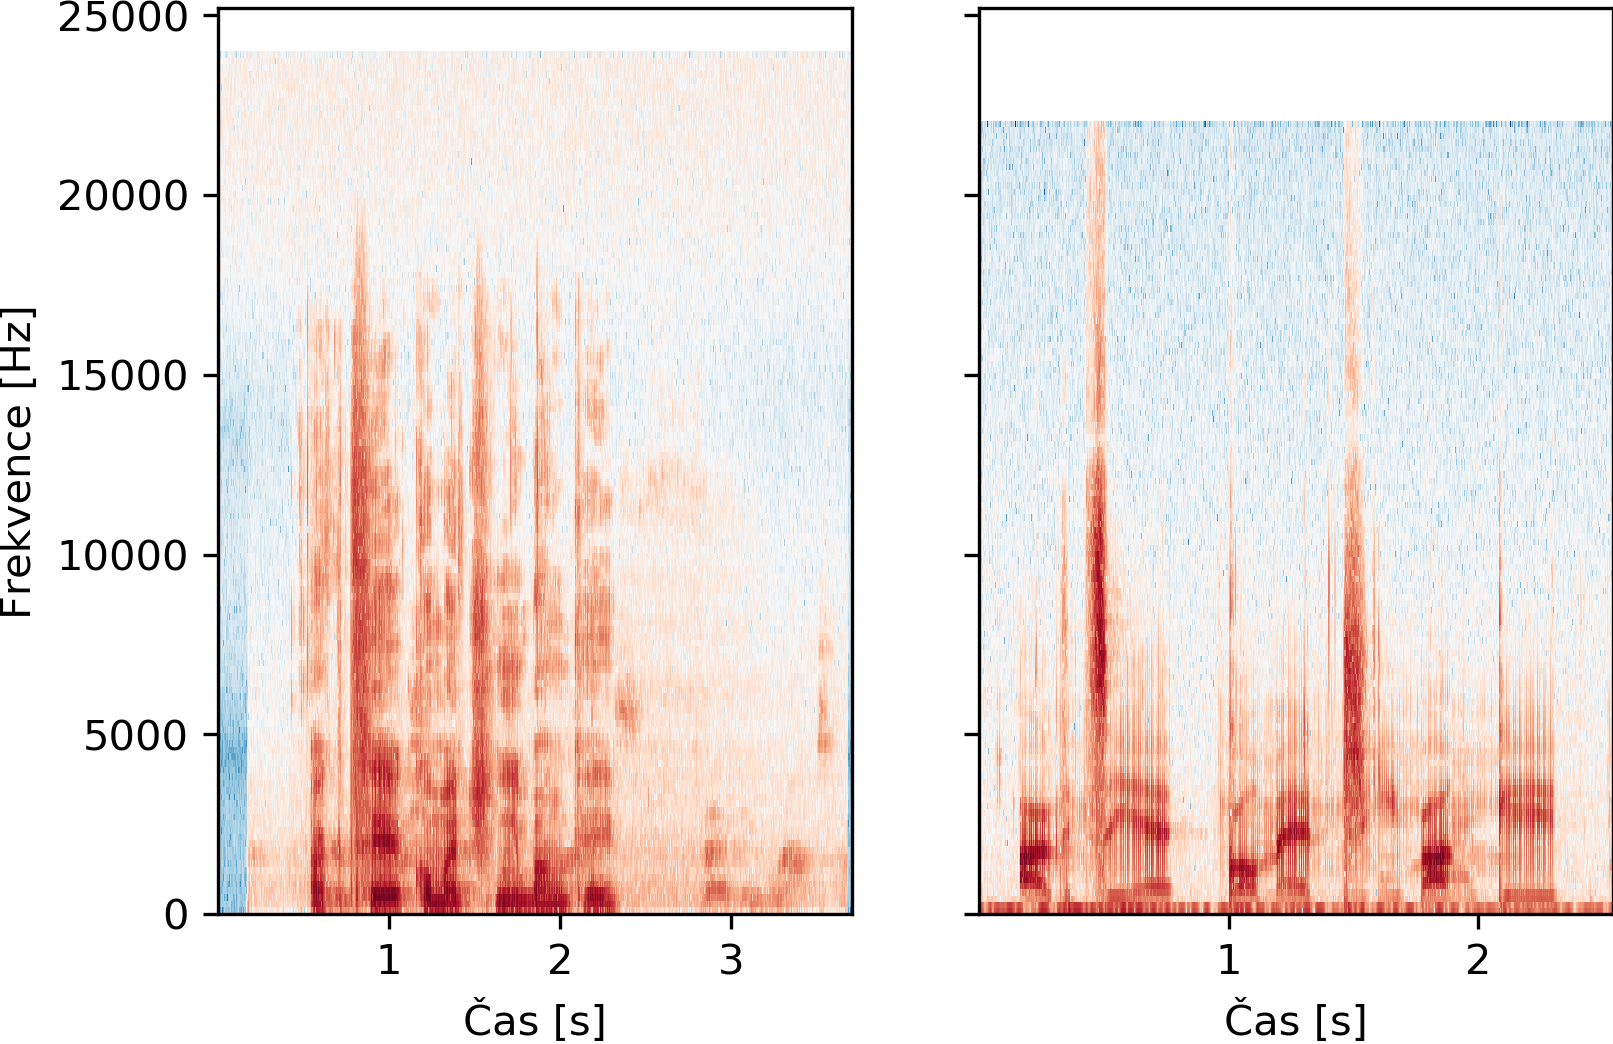
\includegraphics[width=\textwidth]{./ch4-experiments/img/spectrogram_subplot.png}
%   \caption{}
%   \label{}
% \end{figure}

% \csvautotabular{./ch4-experiments/test.csv}

\begin{table}[htpb]
  \centering
  \def\arraystretch{1.5}
  \pgfplotstabletypeset[
    col sep=comma,
    string type,
    columns/model/.style={column name=Model, column type={|c}},
    columns/8k/.style={column name=8 kHz $[\%]$, column type={|r}},
    columns/16k/.style={column name=16 kHz $[\%]$, column type={|r|}},
    every head row/.style={before row={
      \hline
      & \multicolumn{2}{c|}{WER} \\
    },after row=\hline},
    every last row/.style={after row=\hline},
  ]{./ch4-experiments/tabs/01-frequency.csv}
  \caption{Vliv frekvence na kvalitu modelu.}
\end{table}

\begin{itemize}
  \item popis jak byla data získána
  \item informace o datech (frakvenční rozsah, atp.)
  \item prvotní experimenty k určení parametrů modelu
  \item popsat výsledky, výsledky převážně na HTK (HMM + GMM)
\end{itemize}
